\section{PRELIMINARY AND RELATED WORK}

This paper will focus on the use case of an incremental mining, such as streaming data, while reading the full DB only once.

\begin{figure}
  \centering
  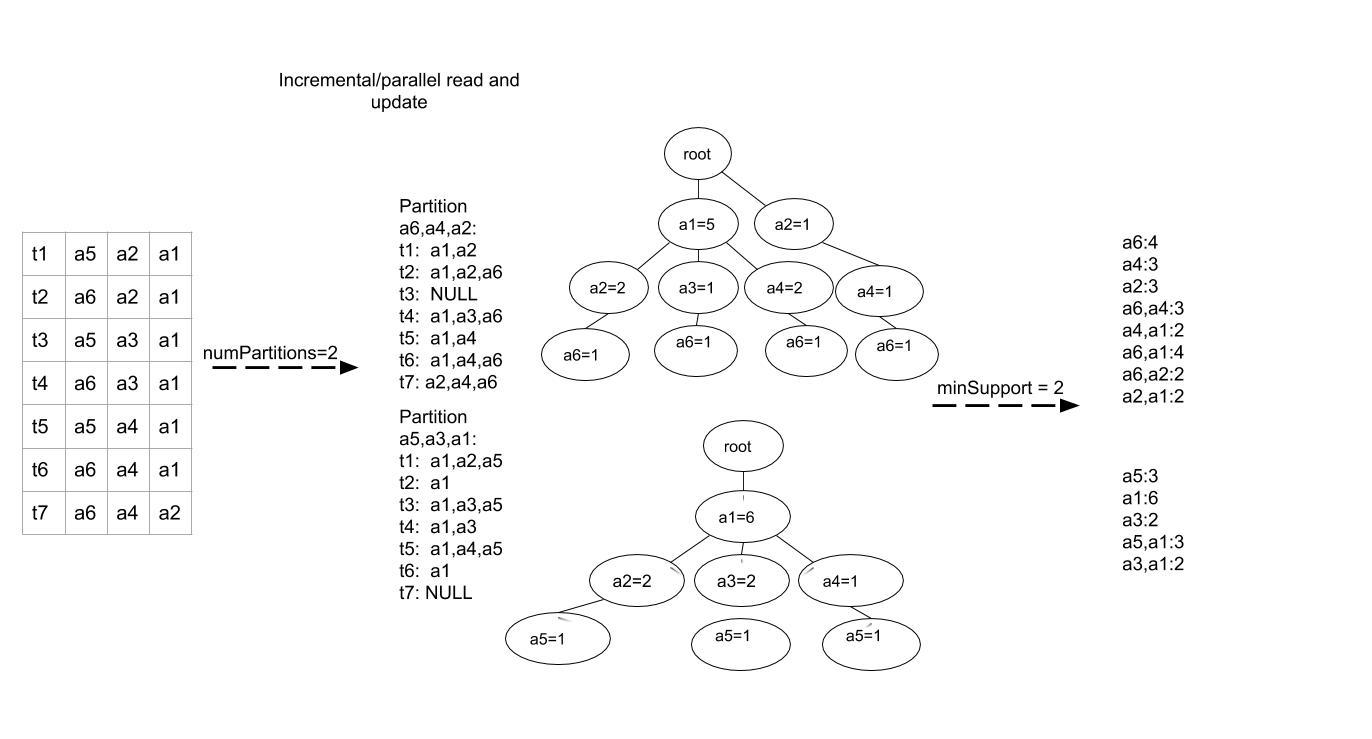
\includegraphics[width=\linewidth]{figures/IncrementalTreeMining}
  \caption{An example of trees and mining for minSup=2 and 2 partitions}
  \label{fig:incrementalParallelMining}
\end{figure}

\subsection{Related Work}
  One of the most well known algorithms for mining association rules is the Apriori algorithm~\cite{agrawal1994fast}. This algorithm is iteratively generating candidates and pruning items with low support at each step. If an item of length N is frequent, then all sub patterns must be frequent as well. Using that idea, an early prune of non-frequent itemsets removes many unnecessary candidates in later iterations.

In the year 2000, a tree based solution was introduced, FPGrowth algorithm and structure~\cite{agrawal1994fast}. This algorithm removes the need for candidate generation and yields better performance~\cite{hunyadi2011performance}. A small example is provided in \autoref{fig:fpgrowthexample}


\subsection{Incremental Frequent Itemsets Mining}
Incremental updates is to recompute outputs which depend on the incoming inputs only, without recomputing the whole data.

The basic challenge in incremental updates for frequent items mining, is a non consistent frequency order. Several algorithms such as AFPIM~\cite{koh2004efficient}, EFPIM~\cite{li2006fast} and FUFP-tree~\cite{hong2008incrementally} are keeping an updated frequency based trees, by reordering branches where frequency has changed.

The work of~\cite{leung2005cantree} presented a Canonical Tree (CanTree) which preserves the frequency descending structure as in FP Growth mining, by relying on a predefined order, which will not affect the tree structure and correctness.

	The work of~\cite{tanbeer2009efficient} proposes an improvement to CanTree, called CompactPattern-Tree, and discusses the memory and computation limitations of CanTree for large incremental Databases. The issues are caused due to un-efficient tree structure, and CP-Tree is proposing an improvement by periodically (using a proposed guideline) updating the order of the construction literals list (l-list) and rebuilding the trees. As mention in the original article and as seen by our experiments, the CanTree and CP-Tree has a similar tree size, and the difference for our test cases was 10\% in tree sizes. However as seen in results of XXX, using semi-frequency based order, improves the mining results by 10X. The reasoning is discussed in section XXX.
	
	

\subsection{Parallel Frequent Itemsets mining}
The difficulty in parallelizing FP-growth is to distribute iterations to parallel trees while still allowing correct mining. PFP~\cite{li2008pfp} is solving this by dividing the DB transactions to independent trees using a Group-List, where every group consists of items, and redistributing iterations in the DB based on this list.
PFP~\cite{li2008pfp} is working in the following steps:

\begin{steps}
	\item Find global frequency list, F-List
	\item Group items G-list
	\item PFP:
		\begin{enumerate}
			\item For each Ti, order by F-List frequency
			\item For each aj in Ti, replace aj with gi that aj belongs to its group
			\item For each gi, if it appears in Ti, find its right-most location in Ti, say L and output:
 <key'=gi; value'={Ti[0]…Ti[L]}>
 			\item Group by key' = gi
 			\item For each group gi, build appropriate tree
 			\item For each group gi, mine the generated tree (filter items not in gi).
		\end{enumerate}
\end{steps}

\begin{figure}
  \centering
  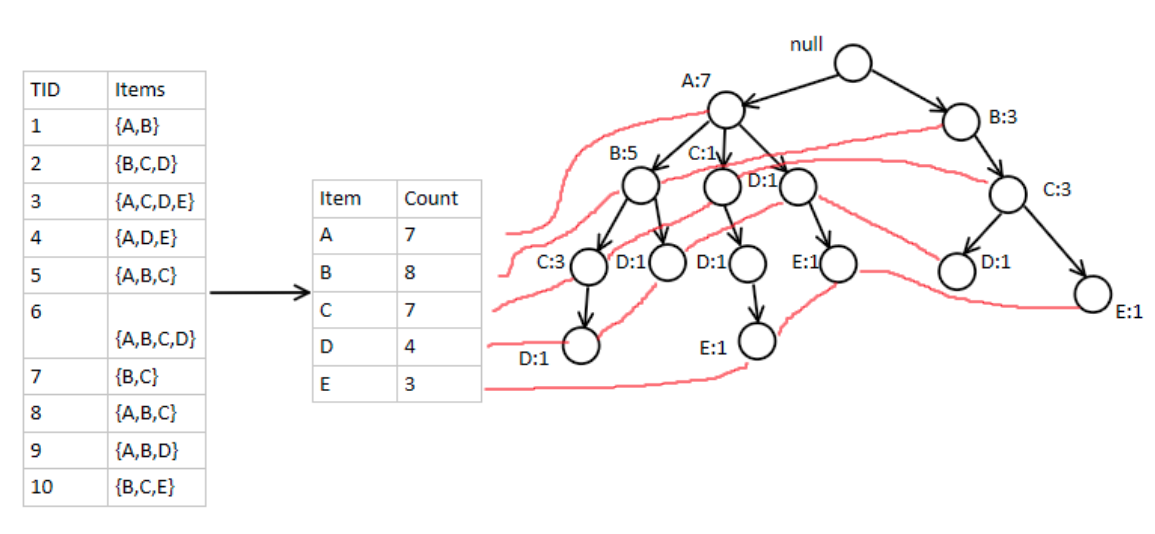
\includegraphics[width=\linewidth]{figures/fpgrowthexample}
  \caption{FPGrowth example}
  \label{fig:fpgrowthexample}
\end{figure}

It is important to mention that there might be some duplicates at several groups of frequent itemsets in stage 3.6, but this is solved when filtering the 1-length items that are not relevant to the specific group. This duplication also affects the size of the generated trees and overall memory.

\subsection{Incremental and Parallel Frequent itemsets mining}

Combining the previous 2 sections, yields an algorithm that does not rely on frequency order and uses parallelism advantages for computations of FIS.
The drawbacks are also drawn from the 2 algorithms - large memory consumption for saving all items and recursively calculating FIS. As we will show later in the results, using an approach similar to ~\cite{kohefficient} and maintaining a pre-min support, together with using a semi-freq-order as in ~\cite{tanbeer2009efficient}, will significantly improve memory and mining runtime results.

